\chapter{Organization Overview}
\label{chapter-2}

\section{Introduction}
\par [Company Name] is a modern firm committed to providing holistic [industry/sector] solutions. With strong commitments to excellence, precision, and customer success, the organization ensures its products, processes, and systems deliver exceptional quality and reliability. Combining technological expertise with industry knowledge, [Company Name] helps clients improve operational efficiency, mitigate risks, and exceed customer expectations.

\section{Company Profile}
\par \textbf{[Company Name]} is a leading [industry] solutions provider helping businesses of all sizes achieve superior performance. Headquartered at [Location], the company is built on core values including integrity, excellence, innovation, and client-centricity. Founded in [Year], it has grown to [Number] qualified employees, offering innovative solutions across [Region/Country].

\subsection{Certifications}
\begin{table}[H]
\centering
\caption{Company Certifications}
\begin{tabular}{|l|p{5cm}|p{6cm}|}
\hline
\textbf{Certification} & \textbf{Details} & \textbf{Significance} \\
\hline
Example 1 & Description & Business impact \\
\hline
\end{tabular}
\label{tab:certifications}
\end{table}

\subsection{Historical Timeline}
\begin{itemize}
    \item Founding and key milestones
    \item Service expansions
    \item Recent developments
\end{itemize}

\subsection{Work Environment}
\par The company fosters a [describe culture] environment with [list key features]. Employees benefit from [mention perks] while management continuously works to improve [mention areas].

\subsection{Mission and Vision}
\begin{itemize}
    \item \textbf{Mission:} Core commitments and value proposition
    \item \textbf{Vision:} Future aspirations and industry goals
\end{itemize}

\subsection{Core Values}
\begin{itemize}
    \item Quality standards
    \item Customer focus
    \item Innovation
    \item Teamwork
    \item Ethics
\end{itemize}

\section{Organizational Structure}

\textcolor{red}{Organizational structure (i.e. Enterprise or Startup, or etc.) and your interactions with various departments, including collaboration with team leads and cross-functional coordination. This involves regular communication with other departments to understand their responsibilities, align on goals, and support interdepartmental workflows effectively.}

\par The company's structure ensures operational efficiency through clear roles and departmental collaboration. Figure \ref{fig:company-structure} shows the hierarchical breakdown.

\begin{figure}[H]
    \centering
    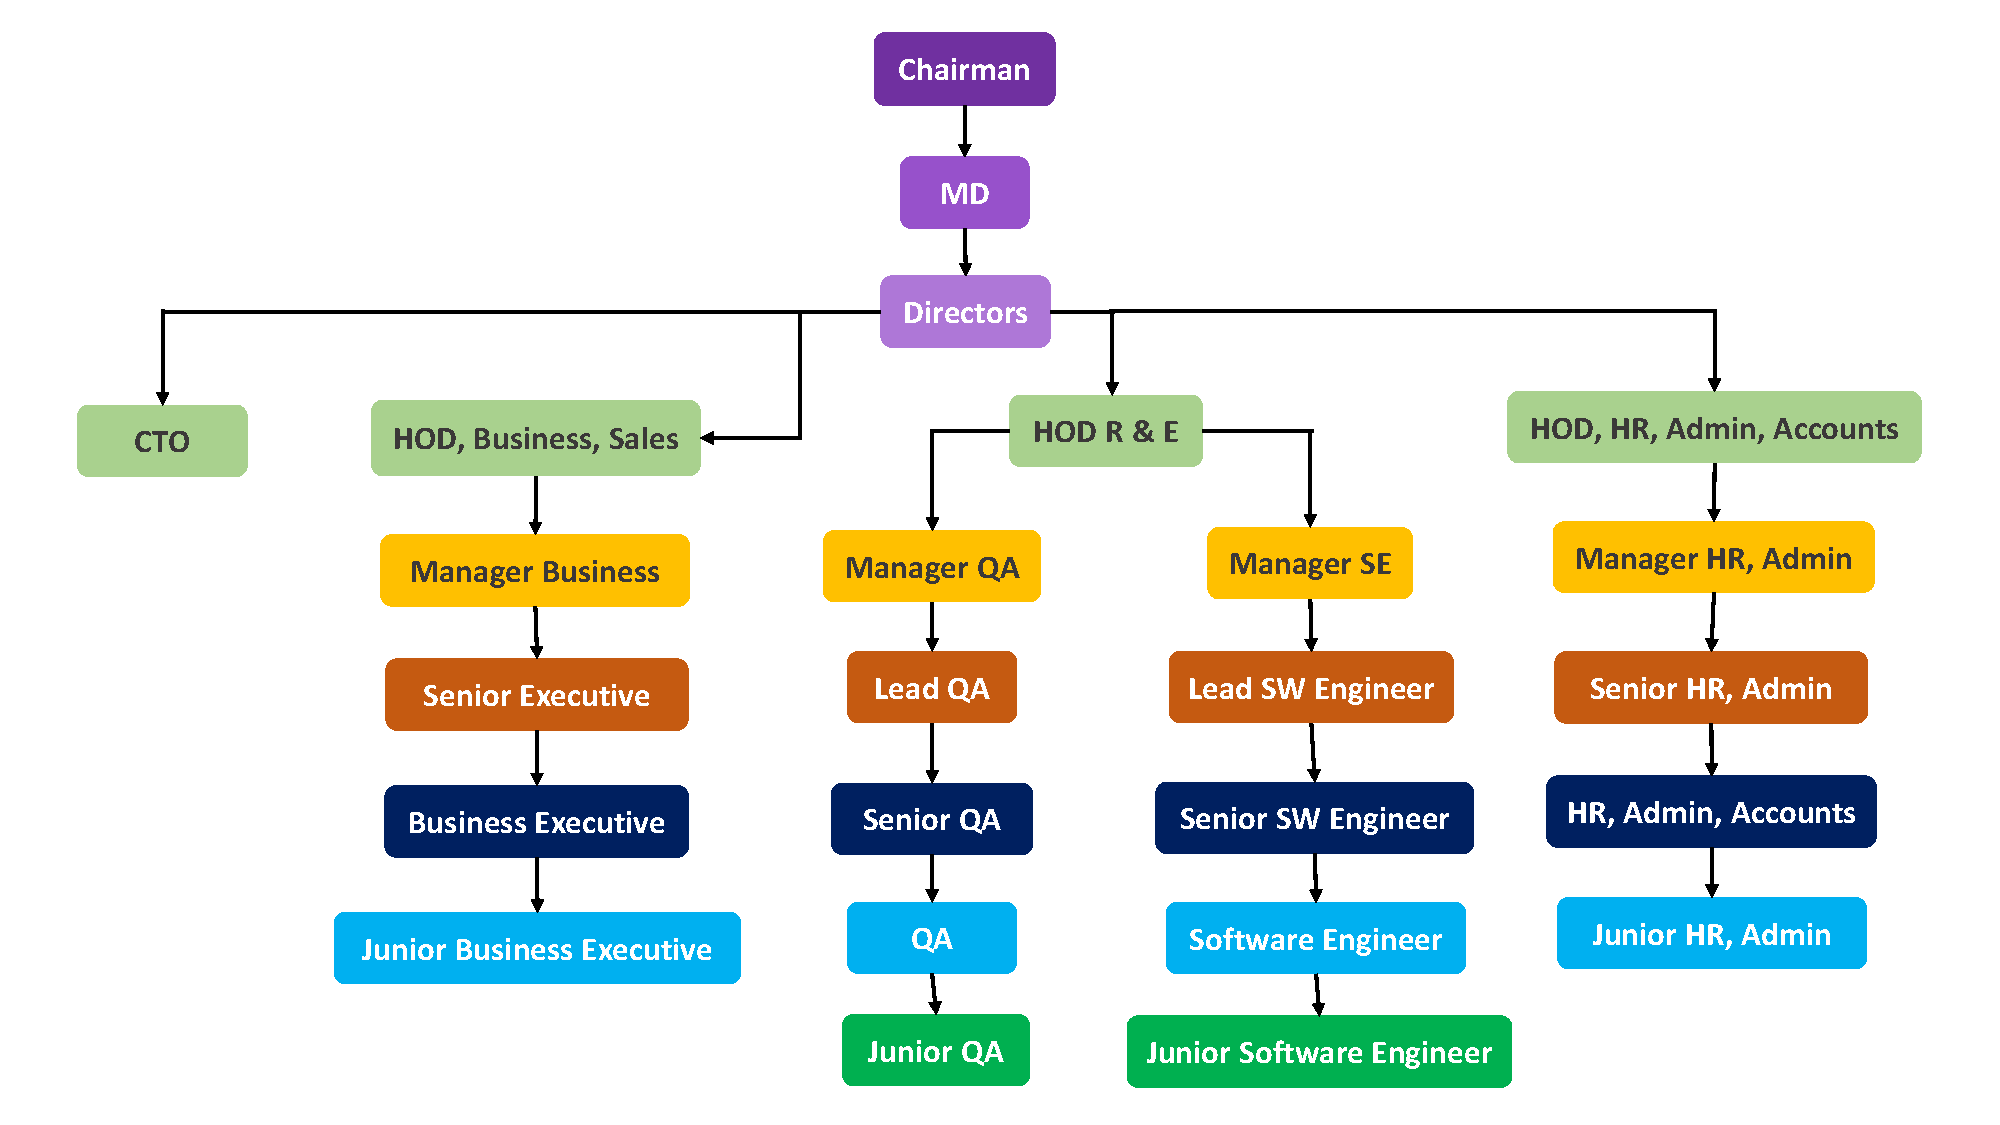
\includegraphics[width=1.0\linewidth]{figures/Company.pdf}
    \caption{Organization Structure}
    \label{fig:company-structure}
\end{figure}

\subsection{Type of Organization}
\par The company operates as a \textit{[Enterprise/Startup/Hybrid]} model, influencing its pace of decision-making, flexibility in processes, and hierarchy depth. This structure defines how projects are prioritized, how resources are allocated, and how quickly initiatives move from concept to execution.

\subsection{Hierarchical Overview}
\begin{itemize}
    \item \textbf{Executive Leadership:} Provides strategic direction.
    \item \textbf{Department Heads:} Lead operational units.
    \item \textbf{Technical Teams:} Implement core solutions.
    \item \textbf{Support Functions:} Handle HR, admin, and finance.
\end{itemize}

\subsection{Roles and Responsibilities of Officials}
\begin{itemize}
    \item \textbf{Chief Executive Officer (CEO):} Sets overall strategic vision, ensures organizational goals align with market opportunities, and represents the company to external stakeholders.
    \item \textbf{Chief Operating Officer (COO):} Oversees day-to-day operations, manages cross-departmental workflows, and ensures operational efficiency.
    \item \textbf{Chief Technology Officer (CTO):} Leads technology strategy, oversees development teams, and ensures that technical solutions meet business requirements.
    % Add other roles as needed
    \newline
    ...
\end{itemize}

\subsection{Interactions with Various Departments}
\par Daily operations involve engagement with multiple departments. Each department has clearly defined responsibilities, and regular communication ensures mutual awareness of progress, challenges, and dependencies.

\subsection{Collaboration with Team Leads}
\par Team leads serve as the primary coordination points within their functional areas. Regular sync meetings, sprint reviews, and project status updates help align technical deliverables with business objectives.

\subsection{Cross-Functional Coordination}
\par Many initiatives span across technical, product, and support teams. Structured workflows—such as shared project boards, standardized reporting formats, and agreed escalation paths—enable smooth collaboration between functions.

\subsection{Interdepartmental Communication}
\par Consistent communication channels, including weekly cross-departmental meetings, collaborative documentation platforms, and direct messaging tools, help maintain alignment and resolve issues before they impact delivery timelines.



\section{Products/Services}
\textcolor{red}{Provide detailed information about a product or service, including its methodology, any relevant diagrams such as ER (Entity-Relationship) diagrams or UI (User Interface) designs. You may choose a product/service that is well-known, widely used, or one you are familiar with.}
\begin{itemize}
    \item \textbf{Details} [General description]
    \item \textbf{Specialized Services:} [General description]
    \item \textbf{Training Programs:} [General description]
\end{itemize}



\section{Clients}
\begin{itemize}
    \item Representative clients across industries
    \item Confidentiality note regarding unnamed clients
\end{itemize}


\section{Direct Involvement of Resources During Training }
\begin{itemize}
    \item \textbf{Human Resources:}
    \begin{itemize}
        \item Mentors and supervisors
        \item Training personnel
        \item Leadership access
    \end{itemize}
    \item \textbf{Technical Resources:}
    \begin{itemize}
        \item Work equipment
        \item Software tools
        \item Testing platforms
    \end{itemize}
\end{itemize}


\section{Constructive Feedback About the Training Program}
\begin{itemize}
    \item Provide balanced feedback:
    \begin{itemize}
        \item Positive aspects of the experience
        \item Areas for improvement
        \item Suggestions for future interns
    \end{itemize}
    \item Maintain professional tone
    \item Focus on learning outcomes
\end{itemize}

\section{Conclusion}
\par [Company Name] is a [type] organization specializing in [key services]. With its [describe structure] and focus on [key values], the company maintains industry standards while contributing to sector growth. The organization's commitment to [highlight principle] makes it an ideal environment for professional development.